\lab{Algorithms}{GMRES}{GMRES}
\label{lab:GMRES}
\objective{In this lab we will learn how to use the GMRES algorithm.}

The GMRES (``Generalized Minimal Residuals") algorithm solves linear systems of the form $Ax=b$ for nonsymmetric matrices that are so
large that either they cannot be stored in memory, or direct methods cannot run to completion in a reasonable time.
It is an iterative method that relies on Krylov subspaces to reduce a high-dimensional problem to a sequence of smaller dimensional
problems.

\section*{The Arnoldi Iteration and Approximate Solutions}
The basic idea of GMRES is as follows.
Let $A$ be an $m\times m$ matrix (real or complex), where $m$ is very large,
and let $b \in \mathbb{F}^m$ ($\mathbb{F}$ may either be the real or complex numbers).
Let $\mathcal{K}_n$ denote the order-$n$ Krylov subspace generated by $A$ and $b$.
In each iteration, we consider the least squares problem
\begin{equation}
\underset{x \in \mathcal{K}_n}{\text{minimize}}\qquad \|b-Ax\|_2.
\label{eq:GMRES_lstsq1}
\end{equation}
Now if $x \in K_n$, then $x$ can be expressed as a linear combination of basis vectors $b, Ab, \ldots, A^{n-1}b$, i.e.
\[
x = y_1b + y_2Ab + \cdots + y_nA^{n-1}b.
\]
If we let $K_n$ be the matrix whose columns are $b, Ab, A^{2}b, \cdots, A^{n-1}b$, then we can write this simply as
$x = K_n y$.
Then the solution of the least squares problem is the vector $K_{n}y$ such that $\|b-A K_{n}y\|_2$ is minimized.
\begin{figure}
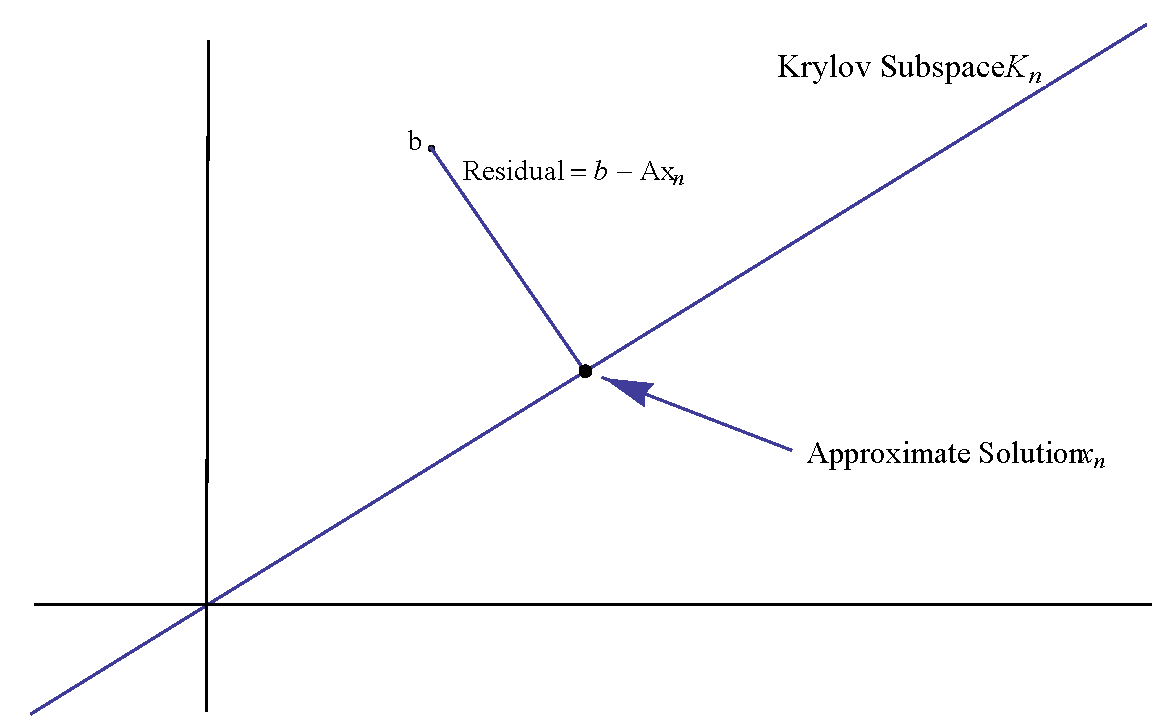
\includegraphics[width=\textwidth]{LeastSquares}
\caption{GMRES involves solving the least squares problem repeatedly.}
\end{figure}

The major drawback of this approach is that it relies on the matrix $K_n$, which tends to be ill-conditioned due to its columns
being far from orthogonal (as discussed in Lab \ref{lab:kry_arnoldi}).
%To see this, suppose there is an eigenbasis for $A$ with associated eigenvalues, and suppose $\lambda$ is the largest eigenvalue.
%Then $\lambda^n$ is an eigenvalue of $A^n$.
%Since $\lambda$ is bigger than the other eigenvalues of $A$, $\lambda^n$ may be much, much bigger than the other eigenvalues of $A^n$,
%which are simply the eigenvalues of $A$ raised to the $n$th power.
%Thus the eigenvector associated with $\lambda$ often begins to dominate as we progress, with the end result being that the columns of
%$K_n$ become nearly linearly dependent.
The easiest fix in this situation is to use the Arnoldi iteration so that we have an orthonormal basis for $\mathcal{K}_n$ to work with.
Not only does this alleviate the problem of ill-conditioning, it also allows us to optimize in other ways, due to the special
structure of the matrices produced.

Let $q_1,\ldots, q_n$ be the orthonormal basis for $\mathcal{K}_n$ obtained by the Arnoldi iteration, and let $Q_n$ be the matrix
having these vectors as its columns.
Recall that $q_1 = b/\|b\|_2$.
Finally, let $H_n$ be the $(n+1)\times n$ upper Hessenberg matrix generated by the Arnoldi iteration, and let $e_1=(1,0,\cdots,0)$.

In this orthonormal basis, $x \in \mathcal{K}_n$ implies that there is some vector $y$ such that $x = Q_n y$.
Further, it is not hard to check that the matrices generated by the Arnoldi iteration satisfy the equation
\[
AQ_n = Q_{n+1}H_n.
\]
We also have the identity
\[
b = \|b\|_2q_1 = \|b\|_2Q_{n+1}e_1.
\]
Putting all of this together, we can rewrite the objective function of our least squares problem as follows:
\begin{align*}
\|b - Ax\|_2 &= \|Ax - b\|_2\\
&= \|AQ_ny - b\|_2\\
&= \|Q_{n+1}H_ny - \left(\|b\|_2Q_{n+1}e_1\right)\|_2\\
&= \|Q_{n+1}\left(H_n y - \|b\|_2e_1\right)\|_2.
\end{align*}

The matrix $Q_{n+1}$ has orthonormal columns, but it does not have enough columns to be a unitary matrix.
Let us extend the set $q_1,\ldots, q_{n+1}$ to an orthonormal basis $q_1,\ldots,q_{n+1},q_{n+2},\ldots,q_m$
of our space, and let $Q'$ be the matrix whose columns are equal to these vectors.
Then $Q'$ is now a unitary matrix, and hence preserves the norm, i.e. $\|Q'z\|_2 = \|z\|_2$ for all $z \in \mathbb{F}^m$.
Given $x \in \mathbb{F}^{n+1}$, if we define $x' \in \mathbb{F}^m$ to be
\[
x' =
\begin{bmatrix}
  x\\
  0\\
  \vdots\\
  0
\end{bmatrix},
\]
then you can easily check that
\[
Q'x' = Q_{n+1}x.
\]
From this, we deduce that
\begin{align*}
\|Q_{n+1}x\|_2 &= \|Q'x'\|_2\\
& = \|x'\|_2\\
&= \|x\|_2.
\end{align*}
Hence, we conclude that
\[
\|Q_{n+1}\left(H_n y - \|b\|_2e_1\right)\|_2 = \|H_n y - \|b\|_2e_1\|_2.
\]
Thus, the least squares problem given by \ref{eq:GMRES_lstsq1} is equivalent to the problem
\begin{equation}
\underset{y \in \mathbb{F}^n}{\text{minimize}}\qquad \|H_n y - \|b\|_2e_1\|_2.
\label{eq:GMRES_lstsq2}
\end{equation}
If $y$ is the solution to this problem, then the solution to \ref{eq:GMRES_lstsq1}, and hence an approximate
solution to $Ax = b$ is given by $x=Q_n y$.

We can measure how good our approximate solution is by considering the residual, which we define to be
\[
\frac{\|Ax-b\|_2}{\|b\|_2}.
\]
We can express this residual in terms of $y$ as follows:
\begin{equation}
\frac{\|H_n y - \|b\|_2e_1\|_2}{\|b\|_2}.
\label{eq:GMRES_residual}
\end{equation}
\section*{The GMRES Algorithm}
To summarize the discussion in the previous section, the GMRES algorithm combines the Arnoldi iteration with linear least squares,
generating successive approximations to the solution of $Ax = b$.
We fully present GMRES in Algorithm \ref{alg:gmres}.

\begin{algorithm}
\begin{algorithmic}[1]
\Procedure{gmres}{$Amul, b, k=100, tol=1E-8$}
	\State $m \gets b.size$						\Comment{Some initialization steps}
	\State $Q \gets \text{empty}\left(m, k+1\right)$
	\State $H \gets \text{zeros}\left(k+1, k\right)$
	\State $q_0 = b/\|b\|_2$
    \For{$n=1,2,\ldots, k$}
        \State Set entries of $Q$ and $H$ as in Arnoldi iteration.
        \State Calculate least squares solution $y$ of \ref{eq:GMRES_lstsq2}.
        \State Calculate the residual $r$ given by Equation \ref{eq:GMRES_residual}.
        \If{$r < tol$}
            \State \pseudoli{return} $Q_ny, \,\, r$
        \EndIf
    \EndFor
    \State \pseudoli{return} $Q_ny, \,\, r$						
\EndProcedure
\end{algorithmic}
\caption{GMRES}
\label{alg:gmres}
\end{algorithm}

%\begin{warn}
%The Python function \li{linalg.lstsq} solves a least squares problem, returning not only the vector, $y$, but also the residual,
%the rank of the matrix, and the singular values.
%Be careful when you write your code that you access the correct results and don't just assume that \li{linalg.lstsq} returns the
%vector that you want.
%The least squares solver also returns a residual, but it's not the number we reference in this book, so be sure to take the square
%root of the residual reported by the solver and divide by $\norm{b}$ to get $res=\norm{Ax-b}/\norm{b}$.
%\end{warn}

\begin{problem}
Implement the GMRES algorithm as presented above. For simplicity, assume that we are only dealing with real-valued matrices and vectors.
Write a function \li{gmres} which accepts a function handle $Amul$ that computes the matrix-vector multiplication $Ax$ for any $x$,
a vector $b$, the maximum number of iterations to perform, and an error tolerance $tol$.
Use the GMRES algorithm to compute an approximate solution to the system of equations $Ax = b$, and return this solution, as well as
the residual.

Assume that the matrix is invertible, and ignore the possibility of dividing by zero for now, as this will occur very infrequently.
You may use the built-in least squares solver in \li{scipy.linalg} to solve the least squares problem, but check the documentation
for its correct use.

The following function generates an $n \times n$ array with randomly distributed real eigenvalues between $-1$ and $1$.
\begin{lstlisting}
import numpy as np
from numpy.random import rand
from scipy import linalg as la
def rand_eigs(n):
    """ Make an nxn array with random eigenvalues between -1 and 1. """
    A = rand(n) * 2 - 1
    X = rand(n, n)
    return la.lu_solve(la.lu_factor(X), (X * A).T, trans=1).T
\end{lstlisting}

Test your algorithm on a $100\times 100$ matrix with random eigenvalues and a random vector $b$ and $tol=10^{-3}$.
Allow only a maximum of 90 iterations.
Don't expect convergence before 90 iterations in this case, for reasons that will be explained shortly.
\label{prob:MyGMRES}
\end{problem}

\section*{Convergence of GMRES}
At the $n$-th iteration, GMRES computes the best approximate solution to $Ax = b$ within the order-$n$ Krylov subspace
$\mathcal{K}_n$.
If $A$ is full rank, then the order-$m$ Krylov subspace is all of  $\mathbb{F}^m$.
Therefore, we are guaranteed an exact solution, up to rounding error, after $m$ iterations.
This is not very useful, however, because $m$ is prohibitively large in practice.
Instead, we hope to converge to a close approximate solution in $n \ll m$ steps.

The convergence of GMRES for reasonably small $n$ depends highly on the eigenvalues of $A$, and we expect rapid convergence whenever
the eigenvalues are clumped together in several places in the complex plane and if the eigenvalues are not too close to zero.
The worst case is when the eigenvalues are uniformly distributed around the origin.
This is, in fact, the reason that the algorithm failed to converge even after ninety iterations in problem 1.
If you come across a problem with such poorly-distributed eigenvalues, it is best to look for another algorithm, such as conjugate
gradient applied to the normal equations (CGN).

\begin{problem}
Instead of testing GMRES on completely random matrices, test it on matrices with ``nice,'' clumped eigenvalues.
Here's one idea of how to design such a matrix for testing.
\begin{lstlisting}
# Generate a random matrix with nice eigenvalues
def rand_clumps(m, q, r):
    """ Generate a random mxm matrix with q distinct groups
    of eigenvalues around different natural numbers. """
    A = rand(m, m)
    Lambda = np.repeat(np.arange(2, q+2), m / q + 1)[:m]
    variation = (rand(m) - .5) * (2 * r)
    Lambda += variation
    Q = la.qr(A)[0]
    return (Q * Lambda).dot(Q.T)
\end{lstlisting}
Constructing a matrix this way often takes much longer than actually running GMRES to get the solution, especially once we
introduce restarts later on in the lab.
Test GMRES on matrices of this kind for $100\times 100$ matrices.
Convergence should now occur in relatively few iterations.
Try out larger matrices and different values of the parameters to see how this algorithm behaves for these kinds of matrices.
\label{prob:GMRESClumps}
\end{problem}

\section*{Breakdowns in GMRES}
One of the selling points of GMRES is that it can't break down unless it has reached an exact solution.
Why is this the case?
Breakdowns can occur as we try to expand to larger Krylov subspaces.
In each iteration, we have already converted $b,Ab,A^{2}b,\cdots, A^{n-1}b$ into an orthonormal set $q_0,q_1,\cdots,q_{n-1}$.
After computing $A^nb,$ we will try to make it orthogonal to each of the $q_i$.
But what if $A^{n}b$ is already a linear combination of the $q_i$? In other words, what if $A^{n}b$ lies in $\mathcal{K}_{n-1}$?
This means that
\[
\mathcal{K}_{n-1}=\mathcal{K}_n=\mathcal{K}_{n+1}=\cdots,
\]
so we have reached an \emph{invariant subspace},
and the algorithm cannot proceed without modification.
It also means that $A^{n}b = c_0 b + c_1 A b + \cdots + c_{n-1}A^{n-1}b$.
Rearranging this, we have that $c_0 b = c_1 A b + c_2 A^{2} b + \cdots + A^{n}b$, so that $b$ lies in $\mathcal{K}_{n+1}$.
Therefore, $b$ lies in $A\mathcal{K}_n$, so the least-squares problem will actually deliver an exact solution, up to rounding errors,
in this case.
To summarize: \emph{GMRES only breaks down when it has found an exact solution}.

\begin{problem}
If necessary, update your solution to \ref{prob:MyGMRES} to deal with breakdowns.
Consider any division by zero cases in your code.  Make the necessary adjustments to avoid any such cases.
\label{prob:GMRES3}
\end{problem}

\section*{Optimizing Least-Squares for GMRES (Optional)}
The Hessenberg structure and the Krylov subspace relations enable us to save time on the least-squares part of the problem if we use QR factorization.
Observe that if $H_n$ can be factored as $Q_n R_n$, where $Q_n$ is not the same matrix as above and $R_n$ is invertible upper triangular, we may solve the least squares problem by simply solving $R_n x_n=\norm{b} Q_{n}^{H}e_1$ via back substitution.
There are two ways in which we can speed up this process.
First, we take advantage of the Hessenberg structure by using the techniques from Problem \ref{prob:givens_hessenberg} in Lab \ref{lab:givens}.
Recall that the technique in this situation was to use Givens rotations to eliminate the subdiagonal elements one at a time.
This process, which was part of a previous lab, reduces the operation count from $O(n^3)$ to $O(n^2)$.
The second speedup comes from the fact that we already know the QR factorization for $H_{n-1}$ from the previous step of the algorithm.
This means that we can simply update the QR factorization from the previous step rather than computing it all over again.
Since $H_{n}$ has only one more column and row than $H_{n-1},$ all we need to do is update the last column by performing all previous Givens rotations on just the last column of $H_n$, which requires only $O(n)$ work.
Then we perform one final Givens rotation on $H_n$ to eliminate the new subdiagonal entry which was not present in $H_{n-1}$.
Thus, the QR factorization of $H_n$ can be reduced from an $O(n^3)$ process to only $O(n)$ using these special techniques.

The back substitution necessary to solve the least squares problem can also be reduced to an operation of $O(n)$.

The speedup from $O(n^3)$ to $O(n)$ is very good, but it can only partially alleviate the problems that come with a problem that is ill-suited for GMRES.
It may still be useful because it allows us to perform more iterations in a reasonable amount of time.
In many situations, the simple technique of the next section will keep $n$ low enough that the optimizations from this section are not critical.
%
% \begin{problem}
% \label{prob:GMRES2}
% (Optional) Modify MyGMRES to incorporate these optimizations, and call this program MyGMRES1.
% Run both programs on a series of five random $100\times 100$ matrices and compare the time each requires.
% Are the gains substantial?
% Try it again matrices of size $1000\times 1000$ or larger, and see how substantial the difference becomes.
% Try the same thing using the techniqes of the next section.
% Explain why the difference in performance is less dramatic this time.
% \end{problem}

\section*{GMRES(k)}
One of the serious drawbacks of GMRES is that it requires a lot of storage.
At step $n$, we need to store $H_n$ and $Q_n$, so the storage is $O(n^2)$.
It is also true that the complexity of the each iteration increases as $n$ increases, a fact that can substantially slow down the process.
If we want the iteration to proceed over many steps, these challenges can become prohibitive, so there is a modification called GMRES(k), or GMRES with restarts, that seeks to alleviate these difficulties by restarting the algorithm, but with an improved initial guess.
It then builds the Krylov subspaces generated by this improved initial guess and repeats the process as many times as needed.
Here's the outline of the algorithm:
\begin{enumerate}
\item \emph{Set} $k$, the maximum number of iterations before memory requirements or complexity are too large
\item \emph{Set} $b$, the initial guess
\item \emph{while} $i<k$ and convergence is not yet reached and the number of times through this while loop is less than a set maximum
\subitem Run GMRES for up to $k$ iterations, starting with initial guess
\subitem If convergence has not yet occurred, \emph{set} initial guess to equal the most recent estimate of the solution
\end{enumerate}

This process keeps storage under control and ensures that each iteration stays fast, but at the cost of reliability.
Thus, when GMRES(k) does converge, it may be much quicker and require less storage than GMRES without restarts, but in situations where the true solution, $x$ is nearly orthogonal to the first $k$ Krylov subspaces, not much improvement is made at each iteration, so convergence is slow or may fail entirely.
This is, however, an important variation of GMRES and is frequently used.

\begin{problem}
Adapt your prior implementation of GMRES to include restarts.
It should also take the additional argument $k$, the number of iterations before restarting.
Test its speed on the special $1000\times 1000$ matrices we constructed to test GMRES and compare its speed to GMRES without restarts.
No general statement can be made about the comparative speed of these two algorithms.
How do they compare in the case of these matrices with $k=10$ and $A$ has dimension $1000\times 1000$?
\label{prob:GMRES3}
\end{problem}

\section*{Industrial-grade GMRES package}
In practice, of course, you will most frequently use GMRES algorithms written by specialists rather than writing your own version.
In python, one option is the function \li{scipy.sparse.linalg.gmres}.
It also includes an option to specify whether restarts are needed.

\begin{problem}
Test your GMRES algorithm against SciPy's GMRES algorithm on random $500\times 500$ matrices, and report any difference on how quickly convergence is reached.
\label{prob:GMRES4}
\end{problem}

\section*{Summary}
In this lab, we developed the mathematical basis for GMRES, practiced implementing and working with the algorithm, and explored several variations and optimizations which, when used in conjunction and in the right situations, make GMRES the go-to algorithm for many, many applications.
Avoid falling into the trap of thinking that GMRES is a universal solution to all systems of equations dilemmas, since we have already seen that even for simple random matrices, GMRES has horrendous performance.
Learning and knowing when to apply a variety of algorithms is key to effective computing with large matrices.
